\chapter{Course Overview and Modeling Strategy}

Higher brain function is a modeling problem before it is a tooling problem. Memory, planning, inference, abstraction, and decision making are all latent processes: we rarely observe them directly, but instead infer them from behavior, neural activity, and task structure. A useful course repository therefore needs space for both careful conceptual writing and executable model-building.

This scaffold is designed for exactly that. The LaTeX notes can hold the conceptual arc of the course, while the Python package can accumulate simulations, optimization experiments, and quick probes of candidate mechanisms.

\section{What makes a model useful?}

A model of higher brain function should do more than fit observations. It should compress behavior into a tractable set of assumptions, explain why certain error patterns appear, and suggest new experiments or interventions. In cognitive and systems neuroscience, this usually means balancing three goals:
\begin{itemize}
  \item computational clarity,
  \item biological plausibility,
  \item empirical testability.
\end{itemize}

\begin{figure}[h]
\centering
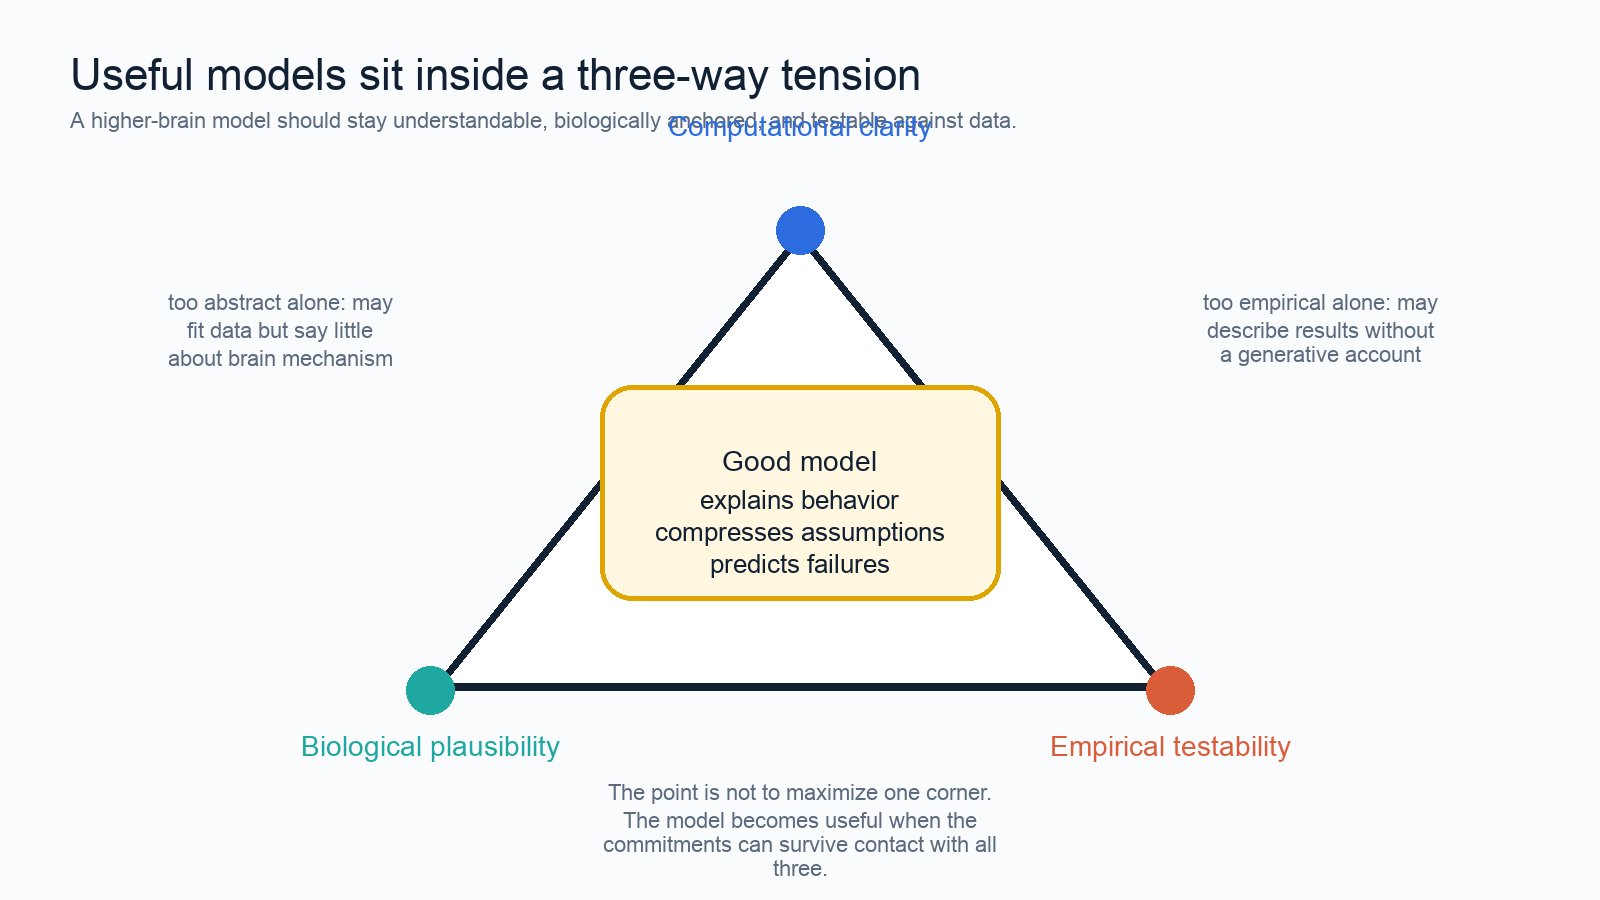
\includegraphics[width=0.82\textwidth]{figures/mhbf-model-triangle.png}
\caption{Why useful models live in tension. Strong higher-brain models stay interpretable, stay anchored to plausible mechanisms, and still make contact with measurable data.}
\end{figure}

\begin{aside}[Practical heuristic]
If a model explains everything equally well, it usually explains nothing. Useful models make sharp commitments about mechanisms, variables, and expected failures.
\end{aside}

\section{A common abstraction stack}

Many courses on higher brain function move across a recurring abstraction ladder: behavior and task structure, latent cognitive variables, circuit or algorithmic mechanisms, and normative or optimization principles.

That ladder connects classical cognitive models to modern neural-network and dynamical-systems viewpoints. The literature on reinforcement learning, attractor dynamics, and recurrent computation makes clear that representation, dynamics, and objective functions must be studied together \parencite{dayan2001theoretical,oreilly2006biologically,wang2008decision}.

\begin{figure}[h]
\centering
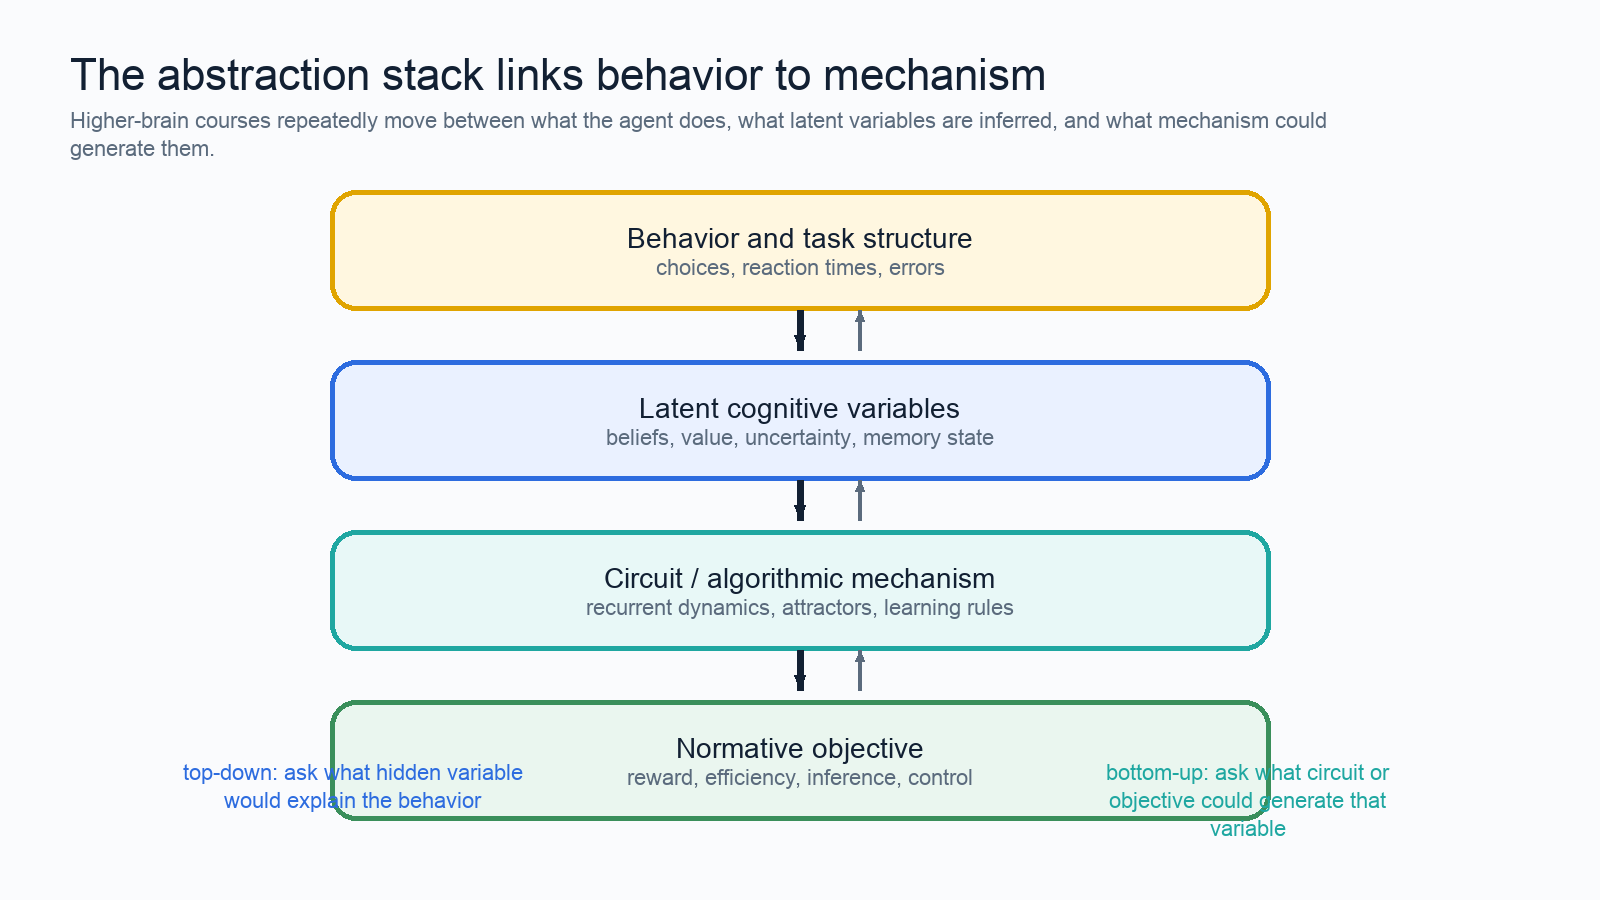
\includegraphics[width=0.82\textwidth]{figures/mhbf-abstraction-stack.png}
\caption{The abstraction ladder used throughout the course. Explanations move downward from observed behavior to hidden variables and mechanism, then upward again to ask whether the mechanism reproduces the behavior.}
\end{figure}

\begin{keyequation}[Generic state-space view]
\[
x_{t+1} = f(x_t, u_t; \theta)
\]
\tcblower
This form is broad enough to include recurrent neural networks, drift-diffusion style updates, working-memory attractors, and many cognitive-state models.
\end{keyequation}

\begin{figure}[h]
\centering
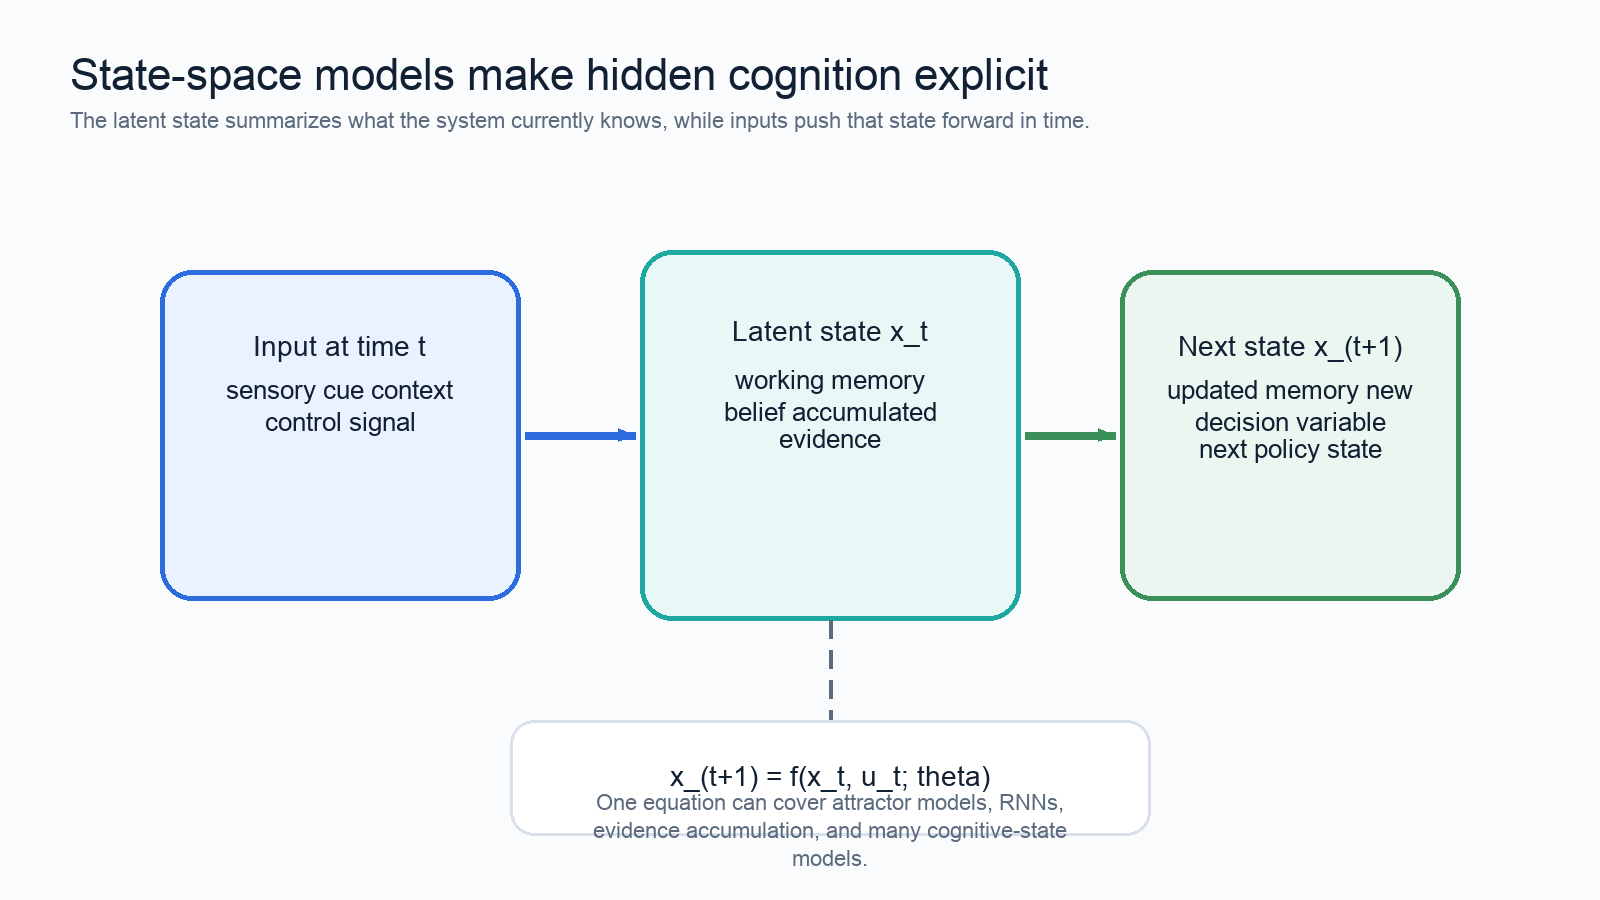
\includegraphics[width=0.82\textwidth]{figures/mhbf-state-space.png}
\caption{State-space intuition. The hidden state carries forward what the system currently ``knows,'' inputs perturb that state, and the update rule determines the next internal configuration.}
\end{figure}

\section{Code organization}

The Python scaffold is deliberately simple. It gives the repository a real package layout immediately, so simulation code and reusable utilities do not end up trapped in ad hoc notebooks. Recommended directions for growth include simulation modules for canonical cognitive tasks, optimization utilities for fitting simple models, plotting helpers for trajectories and phase portraits, and notebook-based reading replications.

\section{Next steps}

Add one chapter per conceptual block, keep derivations in the notes, and let the source package accumulate the minimal reusable code needed to reproduce course figures and experiments. Over time, the repository can become both a reading guide and a computational playground.
